\section{Authentication and authorization}
Authentication and authorization processes are implemented using the secure OAuth 2.0 protocol. The whole procedure is based on communication and data exchange between four roles and components: the resource owner(user) the client app, the authorization server and the authorization microservice.

\subsection{OAuth protocol}
OAuth protocol is a modern industry-standard protocol for authorization. 
In general, the OAuth protocol enables users to provide a client with secure access to server resources and without a need for users to share their credentials directly with an application they want to access. OAuth is widely used by major companies to allow users to grant access to their resources to trusted third-party applications. This protocol is also obviously suitable for university applications and the BI-DBS portal in particular.

\subsection{Tokens} Token in this context a string that has some value for authentication and authorization processes. In the implementation, the client gets the authorization code from the authorization server and exchanges it for access and refresh tokens with the server. 

\subsubsection{Access token}
For representing the authorization in the application the OAuth protocol uses an access token. The access token is a short-time living token that is used to verify the user's access to the application. An access token is sent in every HTTP request sent to the server, so it can verify if the token is valid and then complete a request. It can be used for communication with the application server until that token expires. The expiration time is set to one hour.\\ 
The implementation uses a JWT token type for creating the access token. 
 
\paragraph*{JWT token.} JSON web token(JWT) is a token type standard that allows securely transmitting JSON objects. It consists of three parts: header which specifies the algorithm used to sign the token, payload containing the data being sent and signature that validates the token's integrity and assures it has not been modified.

\begin{figure}[hp]
\centering
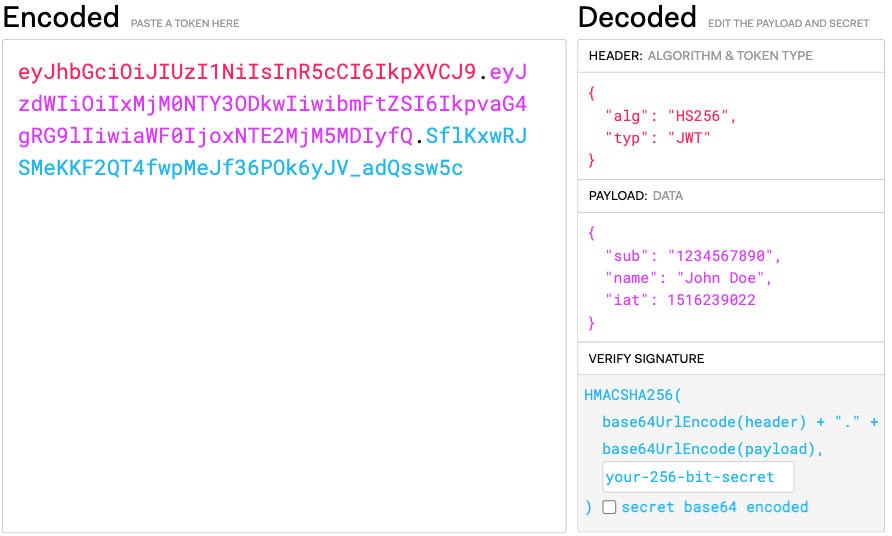
\includegraphics[scale=0.31]{../png/jwt_token.png}
\caption{Example of encoded and decode JWT token from jwt.io.}
\end{figure}



\subsubsection{Refresh token} Refresh token is a type of token used for requesting a new access token when the current one expires. It is a long-time living token, because sue to its existance purpose it is meant to live longer then access token. With a help of refresh token user doe not need repeatedly log in every hour which helps to improve user experience.


\subsection{Authorization server} The authorization server is a key component of the authorization and authentication processes based on the OAuth 2.0 protocol. 
For the authentication and authorization in the BI-DBS portal, we use the faculty's authorization server called Zuul OAAS. It is open-source and available for anybody from CTU. Zuul OAAS provides three endpoints:

\begin{itemize}
    \item \emph{Authorization endpoint: /oauth/authorize.} It is used for the authentication and authorization processes of a user. It displays the login form for a user and after the submission of that form, it validates credentials and in a case of success does a redirect back to the BI-DBS client app server with the authorization code.   
    the authorization code.
    \item \emph{Token Endpoint: /oauth/token.} This endpoint provides us with two important functionalities:
        \begin{itemize}
            \item Exchanging authorization code from the authorization endpoint for access and refresh tokens.
            \item Generating new access token by accepting the refresh token.
        \end{itemize}
   \item \emph{Check Token Endpoint: /oauth/check\_token.} For controlling the validity of the token, the authorization server provides this endpoint which checks the token for being valid.
\end{itemize}

\noindent With the use of these endpoints we have constructed the authentication and authorization processes, which are more deeply described in 4.2.5 and are shown on Figure 4.3.

%https://rozvoj.fit.cvut.cz/Main/oauth2

\subsection{Apps manager} In order to communicate with the authorization server, the application needs to be registered in the Apps Manager. For the further communication with the server we will need three parameters: client id, client secret and redirect URL. The first two parameters are generated by the app manager. These are simplified login and password for our application. But the redirect URL can be set to the URL we want, this URL will be used for the redirect back to our application after the successful authorization of a user. These parameters are used as a part of the HTTP requests, that frontend and backend send to the authorization server.
%https://auth.fit.cvut.cz/manager/app-types.xhtml

\begin{figure}[hp]
\centering
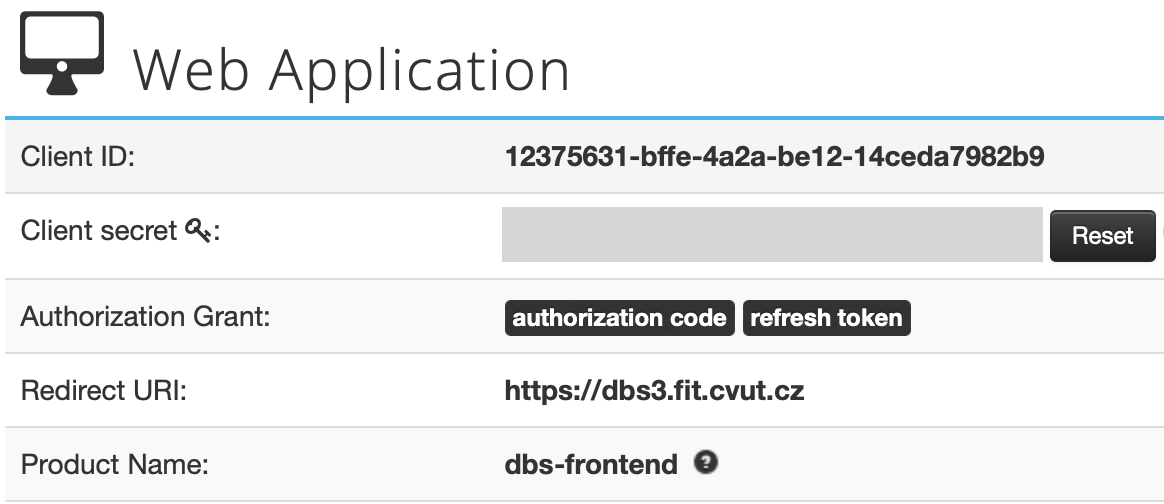
\includegraphics[scale=0.54]{../png/app_manager.png}
\caption{The example of the application registry in the App Manager}
\end{figure}


% \subsection{Authentication and authorization flow}

% \begin{figure}[hp]
% \centering
% 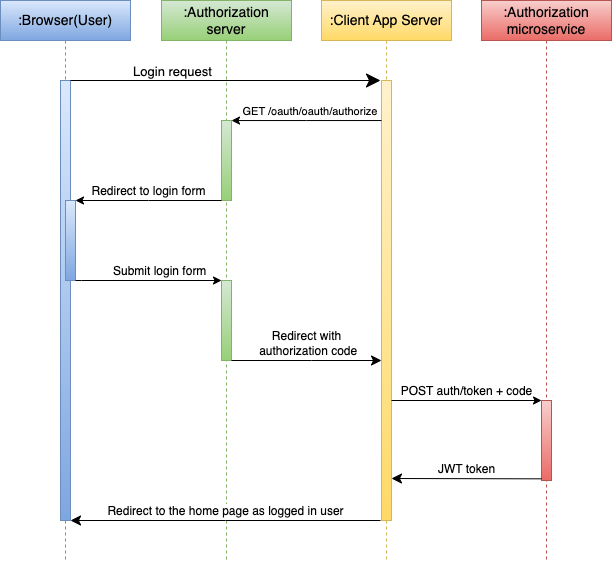
\includegraphics[scale=0.6]{../png/generate_token.png}
% \caption{The example of the application registry in the App Manager}
% \end{figure}


% \subsection{Refresh token flow}


% \begin{figure}[hp]
% \centering
% 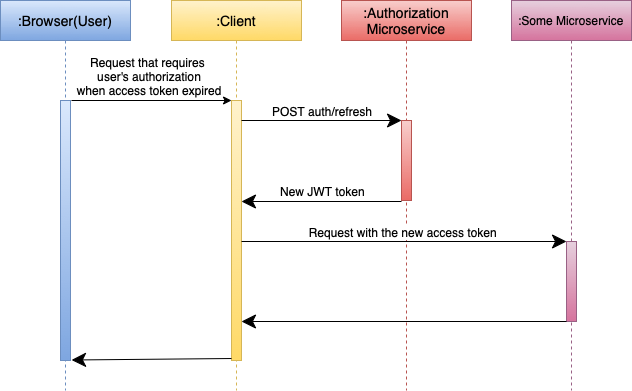
\includegraphics[scale=0.6]{../png/refresh_token.png}
% \caption{The example of the application registry in the App Manager}
% \end{figure}


